% !TEX root = ../main.tex
%
\chapter{Background}
\label{background}
This section introduces some concepts used in this work. First, we define what is stream processing. This is important since it characterizes the behaviour of events collected from data sources under this paradigm. Then, we introduce the Stream Processing Systems (SPS), both the system and its components, and some frameworks used to implement them.


\section{Stream processing}
\label{stream-processing}
%\section{Streaming}
Streaming refers to a continuous flow of data that is generated, transmitted, and processed in real time over a network \cite{Menin2002SMH}. It allows users to access and consume its content as it is under transmission, so there is no need to store all the content before using it. It consists of an external entity sending data to a data processing system. If the service is busy, the data is queued. Generally, streaming is used by web interaction, such as social networking or online playback of multimedia content.

Streaming is largely used in processing information in real-time, when the temporality of the data is relevant, such as online playback of multimedia material. For instance, Streaming API provided by Twitter, can be used to study the most relevant tweets, trending topics or hashtags for specific cases such as election campaigns or natural disasters. Streaming is processed by SPSs.

\begin{figure}[ht!]
  \centering
    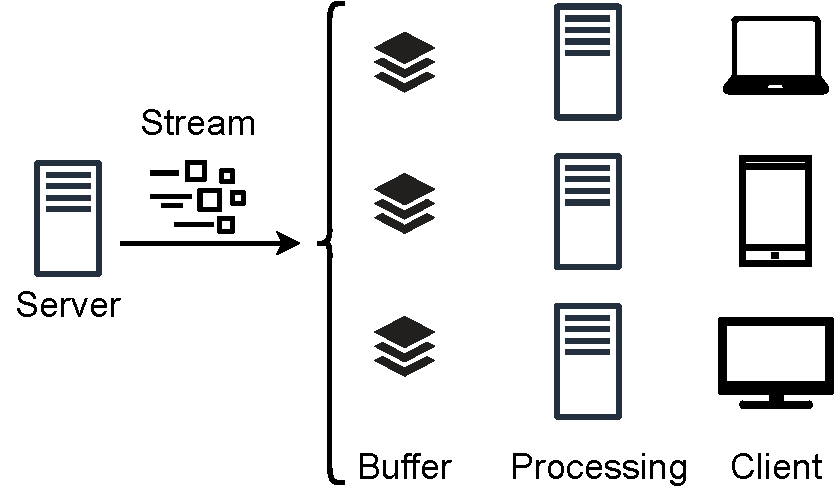
\includegraphics[scale=0.6]{figures/concepts/Streaming.pdf}
  \caption{Streaming example among server and clients.}
  \label{fig:streaming}
\end{figure}

Figure \ref{fig:streaming} shows a server emitting a data stream, which is received by different clients. Each client is in charge of processing the received data, if the client is busy, data is buffered. Otherwise the client will process the data according to the service policy.

%\section{Stream processing}

Stream processing is a computing paradigm and data processing approach that involves the continuous processing of data as it is generated and ingested in real-time. This paradigm focuses on programming applications that can process information on the fly as close to real-time as possible, using system resources in a parallel or distributed manner to meet their objective. It is typically used for real-time applications that close to real time responses, such as monitoring, fraud detection, and predictive maintenance.

Figure \ref{fig:stream-processing} presents a Stream processing scenario. The input stream corresponds to the input stream of external data, which is delivered by an external source such as sensors, log records, or database transactions. Each data is a basic unit, which is processed to obtain relevant information. The stream process is the component in charge of processing the input stream.
These processes can be stateful, so if necessary, the processing status is stored in an external database. It is also possible to process several data in parallel, either using more logical or physical resources. The output stream is the processed data, which can be used as a data stream to be processed or stored.

\begin{figure}[ht!]
  \centering
    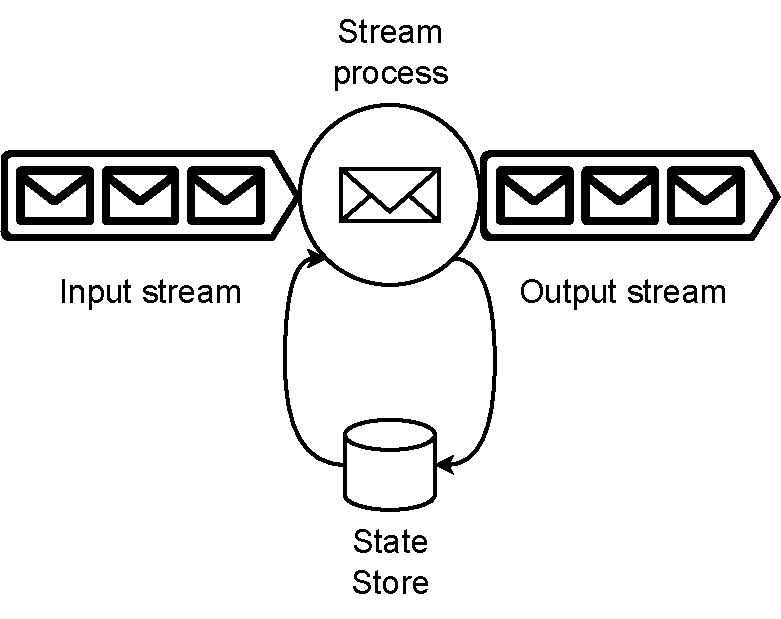
\includegraphics[scale=0.6]{figures/concepts/StreamProcessing.pdf}
  \caption{Stream processing paradigm.}
  \label{fig:stream-processing}
\end{figure}

For the correct functioning of these applications, some requirements should be satisfied. The work \cite{andrade2014fundamentals} defines them, which are classified as follows:

\begin{itemize}
	\item \textbf{Processing large quantities of distributed data}: One of the main goals of Stream processing is the processing of large volumes of data, which are sent in a distributed manner by external sources. By processing these data, the system can monitor, analyse, or control them in real-time, since the data processing is performed as the data stream continues.
	\item \textbf{Addressing stringent latency and bandwidth constraints}: This point refers to a stable connection between components over the network, where bandwidth or latency is not a limiting factor for data processing. Such a requirement is important since an application that considers data in real time is useless if it presents a high latency. Low latency should always be maintained, so that the data is as close to real time as possible.
	\item \textbf{Processing heterogeneous data}: A standard both in the data structure and its format should be application in the raw data from external sources that are used in the Stream processing. In this way, the processing will be homogeneous for all data, avoiding problems associated with the data structure.
	\item \textbf{Providing long-term high availability}: SPS operators can fail which inducing the decrease of data throughput. Thus, it is important to have a fault tolerance mechanism to reduce the loss of information. In the order, provide a constant processing of data, which is stable and persistent over time. Otherwise, information can be lost, compromising the accuracy of the results and requiring more time to collect the lost information or reach a similar state.
\end{itemize}

\section{Stream Processing Systems}
A Stream Processing System (SPS) is a software or framework designed to process and analyze data streams in real-time, which is based on the concepts of Stream processing. The main goal of an SPS is to process high volumes of data in a distributed way and in real-time \cite{kleppmann2016making}. In contrast to the traditional batch processing model, which stores the data to later process it offline \cite{HawwashN14}. SPS shift involves the analysis of data without requiring storage.

The paradigm used by SPSs is based on a directed acyclic graph (DAG) as shown in Figure \ref{fig:sps-concept}. The operators correspond to the vertices of the graph, such as analyzers, word filters or some particular algorithm, while the edges correspond to the dataflow between operators \cite{Shahrivari14}. In addition, the input data (the source) is originated by an external entity, such as streaming from social networks, statistics from the monitoring of a system, or transactions in the stock exchange. The first operator consumes data from the source \cite{AppelFFB12}. In most graphs, the terminal operators are in charge of storing the results of the data processing in a database.

\begin{figure}[ht!]
  \centering
    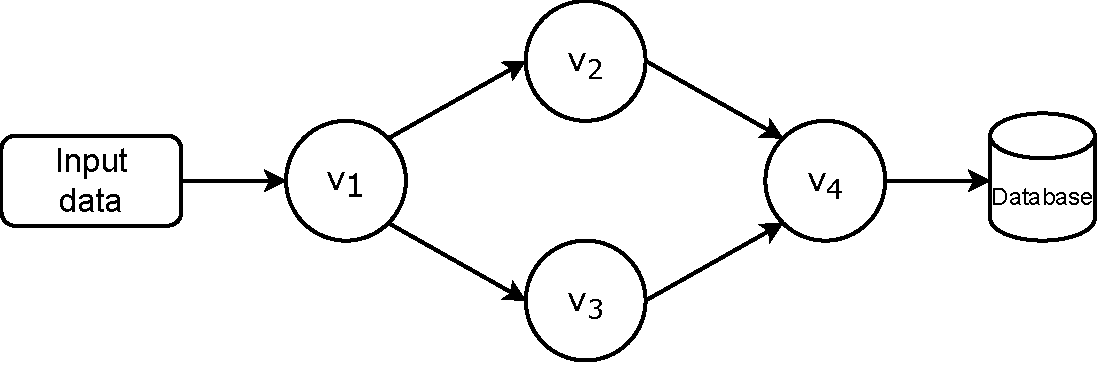
\includegraphics[scale=0.6]{figures/concepts/SPS-Concept.pdf}
  \caption{Example of the representation of the DAG in an SPS application.}
  \label{fig:sps-concept}
\end{figure}

It should be noted that SPSs are distributed, i.e., each vertex is hosted in a physical node available in the environment where the system is hosted, either a \textit{cluster}, a \textit{grid} or a \textit{cloud}. To achieve communication between the operators, systems specially designed for this type of task are used, such as Apache ZooKeeper \cite{HuntKJR10}. The latter consists of a centralized orchestration that maintains configuration and synchronization information of the distributed applications. To this end, each processing node must register in the system, and it is the orchestrator that is subsequently in charge of synchronizing the nodes available for processing and distributing the events among them.

Most applications running on SPS, manage large amount of data, which must be processed to obtain information or statistics, as , for instance, fraud detection, collection of information in case of disasters or analysis of interaction in social networks. To perform real-time processing of the data, \cite{StonebrakerCZ05} establishes the following requirements:

\begin{itemize}
		\item \textbf{Keep the Data Moving}: To ensure low latency in the processing of high volumes of data, it is necessary to preclude the storage of the data when processing it, since the storing data adds unnecessary latency to the system. Thus, the aim is to process data "in-stream", i.e., as the data is received, it is processed.
        \item \textbf{Query using SQL on Streams}: To reduce the development and programming time of projects, it is important to provide an abstraction in the operations performed by the program, as done by a high-level language such as SQL. In this way, there is a set of default functions, which we can be use to query, group, join, or modify, accepted by most popular DBMS. Thus, providing a support to  StreamSQL, a variant of SQL designed for SPS, ends up being an important tool for the SPS ecosystem.
        \item \textbf{Handle Stream Imperfections}: Because data are processed in-stream, it is necessary to provide a provision model for handling data that is delayed, missing, or out-of-order. Hence, if the SPS is performing an operation that considers a calculation in a time window, a mechanism must be provided to handle delayed or out-of-order events. On the other hand, if the system is waiting for a missing data, which might never arrive, then a timeout mechanism should avoid that the system blocks forever.		        
        \item \textbf{Generate Predictable Outcomes}: SPS can predictably process data, always given the same results. This means that the process must be deterministic and repeatable. Such a behaviour reflects the fault tolerance provided by the SPS, given that in the case of data loss, data recovery is possible and the result remains the same.
		\item \textbf{Integrate Stored and Streaming Data}: Some applications may be composed of stateful operations. For instance, the word-counting operator requires variables that store the statistics of the incoming stream. Therefore, the SPS must provide a system for storing, accessing and modifying the states used by the application. These states can also be added to the data in the stream, so it is important to
have a uniform language to deal with both components.
        \item \textbf{Guarantee data security and availability}: SPS must provide data fault tolerance mechanism to ensure data integrity and provide integrity to the processing of critical data information. In this way, the system must provide checkpoint management for both data integrity and state. Thus, in case of data processing failure, the system will be able to reprocess data. 
		\item \textbf{Partition and Scale Applications Automatically}: The distribution of an SPS is important both in terms of scalability and cost. By using the system on a single machine, resource constraints are likely to happen. Likewise, the costs associated with distributing a system across multiple machines are higher. Therefore, the SPS should ideally provide a transparent and automatic distribution of operators on the available machines, providing scalability in its processing.
       \item \textbf{Process and Respond Instantaneously}: When considering the use of SPS, a system is required to respond close to real-time. Therefore, the SPS must provide a solution that copes with operator overloads, which affect system performance. The solution should present low overhead, i.e., small implementation cost or resources requirements, increasing, thus, the efficiency and performance of the system.
\end{itemize}

\subsection{Stream}

Stream is a continuous flow of data records or events that are processed and analysed in real-time. It represents a sequence of data elements that arrive continuously over time. Stream is the fundamental building blocks in SPS corresponding to the input and output channels for data processing. They can represent various types of data, such as sensor readings, log entries, financial transactions, social media updates, or any other type of event-based data.

Streams in SPS typically exhibit the following characteristics \citep{SilvaFBHCG13}:

\begin{itemize}
\item \textbf{Continuous flow}: Streams are continuous and persistent, with data flowing continuously over time. Data arrived are generated, transmitted, and added to stream, creating a dynamic traffic.

\item \textbf{High data arrival rate}: In Streams usually data arrives at a high rate or frequency, requiring SPSs to handle and process data in real-time or near real-time to keep up with the incoming data.

\item \textbf{Potentially unbounded}: Streams can be unbounded, meaning that there is no predefined endpoint or limit. They can continue indefinitely, and the processing system needs to handle the continuous arrival of data without assuming an end.

\item \textbf{Ordered or unordered}: Streams can be ordered, where the order of events is meaningful and needs to be preserved during processing. On the other hand, if the order of events is not important, processing can occur independently on each event.

\item \textbf{Potentially partitioned}: In distributed stream processing systems, streams can be partitioned into multiple partitions or shards. Each partition contains a subset of the data, and, thus, for parallel processing across multiple nodes or processing units can take place.
\end{itemize}

Streams are the primary input to SPS, and then they are ingested, processed, and transformed by various operators or computations. The processed results or derived streams can also be emitted as outputs for further processing, storage, visualization, or integration in other systems.


\subsection{DAG}
A directed acyclic graph (DAG) defines the processing logic of the SPS where each vertex represents an operator, and unidirectional edges (arcs) represent the dataflow. The DAG is defined as $G=(V,A)$, where $V$ is the set of vertices and $A$ is the arcs group. Likewise, $n$ represents the number of vertices in $V$ and $m$ represents the number of arcs in $A$. Each vertex corresponds to an operator, and each arc corresponds to a stream in the SPS application. For example, Figure \ref{fig:sps-dag} shows a DAG, where $G=(V,A)$ with $V=\{\text{v}_1,\text{v}_2,\text{v}_3,\text{v}_4\}$ and $A=\{\text{a}_1,\text{a}_2,\text{a}_3,\text{a}_4,\text{a}_5\}$, $n=4$ and $m=5$. In this case, the initial vertex is $\text{v}_1$ and the terminal vertex is $\text{v}_4$.

\begin{figure}[ht!]
  \centering
    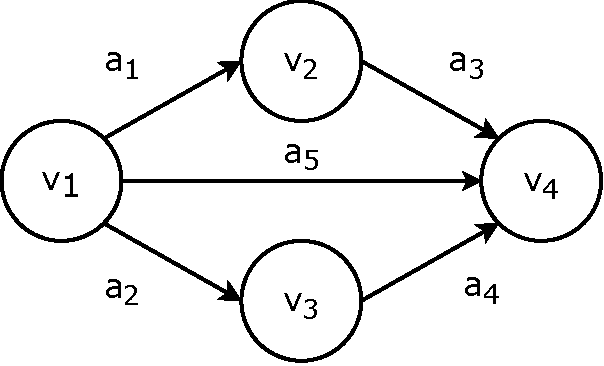
\includegraphics[scale=0.6]{figures/concepts/SPS-DAG.pdf}
  \caption{DAG in an SPS.}
  \label{fig:sps-dag}
\end{figure}

A path $v$ is a sequence of vertices and arcs defined as $v=\text{v}_i\text{a}_k\text{v}_j...\text{v}_p\text{a}_l\text{v}_{q}$, where $\text{v}_i, \text{v}_j, \text{v}_n, \text{v}_m \in V$ for $i,j,p,q \in \{1,...,n\}$ and $\text{a}_k=\{\text{v}_i,\text{v}_j\}, \text{a}_l=\{\text{v}_p,\text{v}_q\} \in A$. Therefore, since in DAGs there are no cycles, the first and last vertices in the path are not the same, i.e., $\text{v}_i \neq \text{v}_q$. For example, in the Figure \ref{fig:sps-dag} it is possible to trace a path between $\text{v}_1$ and $\text{v}_4$, defined by $v_1=\text{v}_1a_1\text{v}_2a_3\text{v}_4$, $v_2=\text{v}_1a_2\text{v}_3a_4\text{v}_4$ or $v_3=\text{v}_1a_5\text{v}_4$, without having cycles.

For a DAG $G=(V,A)$, it is possible to associate the relation $\le$ defined by: for any pair of vertices $(\text{v}_i,\text{v}_j) \in v$ for $i, j \in \{1,...,n\}$ , $\text{v}_i \le \text{v}_j$ if there exists a path $v$ from $\text{v}_i$ to $\text{v}_j$ in $G$. In this way, a topological ordering of $G$ is defined as a list $(\text{v}_i,...,\text{v}_j)$ of vertices of $G$ for $i,j \in \{1,...,n\}$, such that if $i \le j$, then there is no path between $\text{v}_j$ to $\text{v}_i$. For example, Figure \ref{fig:sps-dag} has the list $(1,2,3,4)$ or $(1,3,2,4)$. The ordering is unique, only in the case that a path connects all the vertices, and corresponds to the order in which the vertices appear.

Paths can start from different vertices. Thus, depending on its origin, the set of vertices of different paths is not the same. Figure \ref{fig:sps-dag-complex} presents a complex DAG, where there are two initial vertices ($\text{v}_1$ and $\text{v}_5$) and two terminal vertices ($\text{v}_4$ and $\text{v}_7$). In the case of choosing $\text{v}_1$ as the initial vertex, it is possible to end at $\text{v}_4$ or $\text{v}_7$, but not in the case of $\text{v}_5$, since it can only end at $\text{v}_7$. By taking different paths, the application relies on different operators, so processed data also varies.

\begin{figure}[ht!]
  \centering
    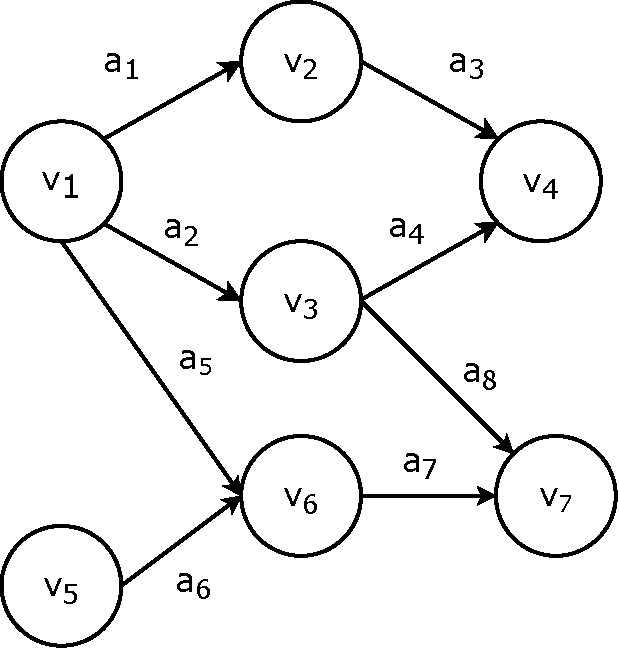
\includegraphics[scale=0.6]{figures/concepts/SPS-DAG-Complex.pdf}
  \caption{DAG complex in an SPS.}
  \label{fig:sps-dag-complex}
\end{figure}

\subsection{Tuples}
The SPS must process structured input data. Therefore, initial operators are used to structure the input data, which can be structured, semi-structured or unstructured. Thus, each structured data created by an external data source is called tuple. A tuple is a basic unit of data that is defined by \textit{(key, value)}, a set of attributes or fields, which flow through the application graph. Each tuple is a single event in the data stream, which is often used to represent an event such as sensor reading, user action, or a financial transaction in real-time applications such as monitoring, alerting, or fraud detection. In general, a tuple has the timestamp of its creation, as well as the timestamp of its predecessor vertices in the DAG. The number and type of attributes in a tuple depend on the need of the application, as well as the path taken by the tuple.

\begin{figure}[ht!]
  \centering
    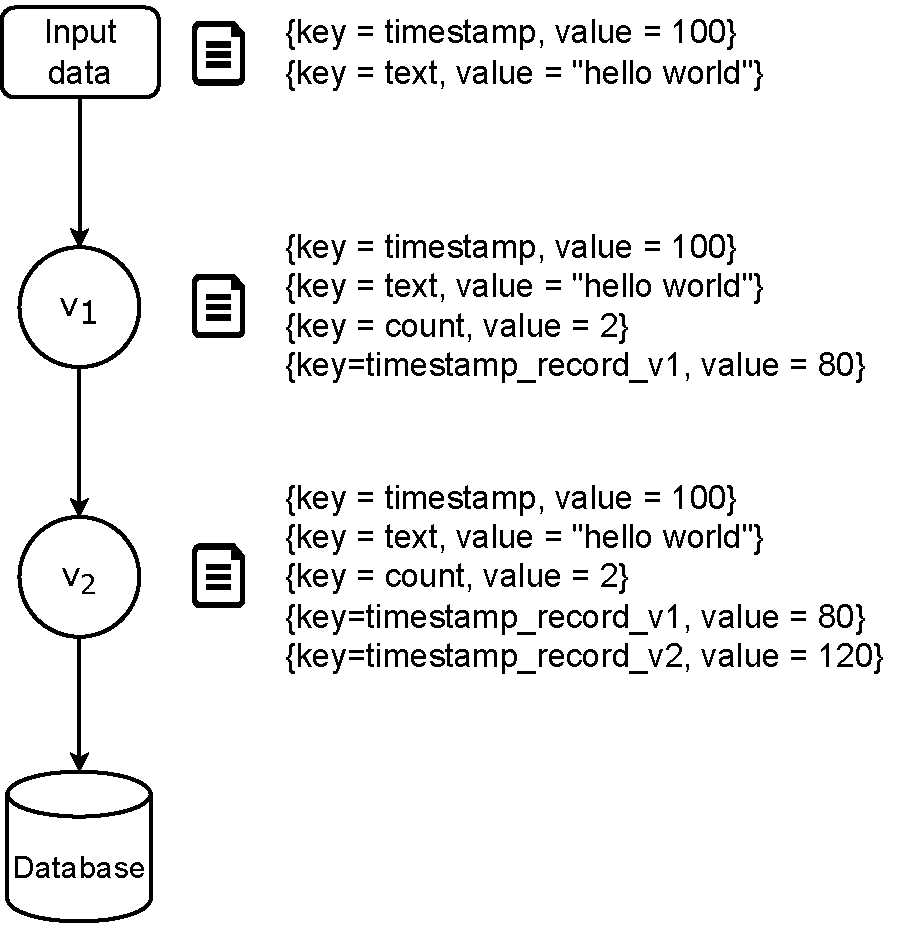
\includegraphics[scale=0.6]{figures/concepts/SPS-Tuple.pdf}
  \caption{The tuple exchange in an SPS.}
  \label{fig:sps-tuple}
\end{figure}

Figure \ref{fig:sps-tuple} presents the flow of a tuple through SPS application, which is defined by four components: input data, two operators and a database. Operator $\text{v}_1$ counts the number of words in the stream, and operator $\text{v}_2$ stores the tuples in a database. The start of the flow begins with the input data, structured in key-value. After this, the tuple is sent to operator $\text{v}_1$, which determines that the number of words is 2. Therefore, it adds a new field \texttt{count} to the tuple and the timestamp record, and sends it to operator $\text{v}_2$. Finally, the $\text{v}_2$ operator stores the tuple in a database, adding the timestamp record.


\subsection{Operator}
An operator is a processing unit that receives data from one or more input streams, performs some computation on the data, and produces one or more output streams. An operator is represented by a vertex in the DAG. The majority of operators are designed to perform light tasks, nevertheless, they can also implement complex tasks, depending on the design of the SPS application.

Depending on the DAG, operators can be replicated and the income data is processed in parallel. Also, each operator has a level of parallelism, which is related to the SPS implementation. Same solutions propose to associate parallel unit to logical resources (i.e. processes or thread), and others to physical resources (i.e. containers or VM).

Figure \ref{fig:sps-operator-parallelism-dag} shows the DAG for an SPS application. The DAG is composed of three operators: $\text{v}_1$, $\text{v}_2$ and $\text{v}_3$. Due to the complexity of operator $\text{v}_2$, the application requires increasing the parallelism of the operator. Figure \ref{fig:sps-operator-parallelism-logical} shows the parallelization of the operator $\text{v}_2$, where $k$ replicas of the operator are created to process data in parallel.

\begin{figure}[!ht]
\begin{center}
\subfloat[Representation by DAG.]{
  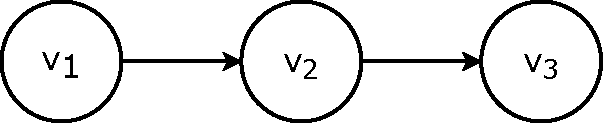
\includegraphics[scale=0.55]{figures/concepts/SPS-Operator-Parallelism-DAG.pdf}
  \label{fig:sps-operator-parallelism-dag}
}

\vspace*{0.5cm}

\subfloat[Representation of operator parallelisation.]{
	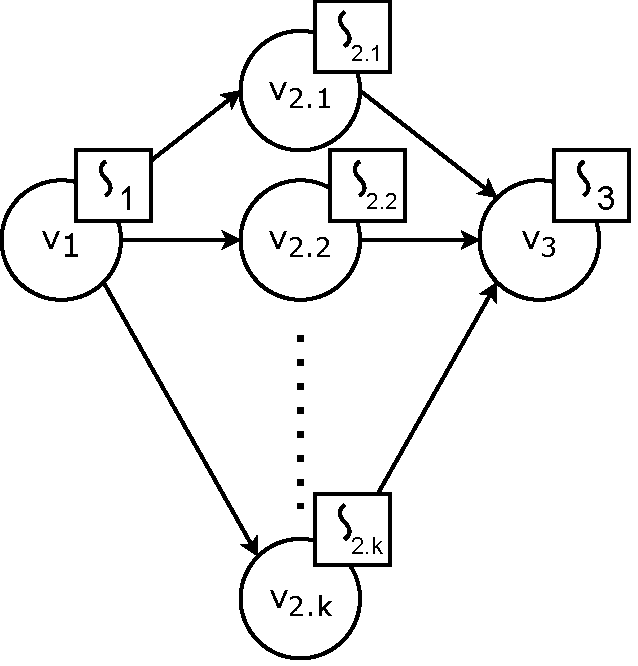
\includegraphics[scale=0.55]{figures/concepts/SPS-Operator-Parallelism-Logical.pdf}
    \label{fig:sps-operator-parallelism-logical}
}
\caption{Example of parallelism of an SPS operator.}
\label{fig:sps-operator-parallelism}
\end{center}
\end{figure}

Data is represented by tuples, so operators process tuples. Depending on the operator's task, tuples are sent without or with modification. It is also possible to discard them, create new tuples, or on the other hand, to perform some analysis on them. Futhermore, depending on whether or not the operator maintains the state or context of the data it processes, operators are classified into: \textit{stateless} and \textit{stateful}.

Stateless operators do not maintain the internal state or context of the data. They are independent tasks that depend only on the input tuples, without the need to know the past processing or global state of the application. These types of operators are used to perform operator-specific tasks. Stateless operators are associated with mapping, filtering, and data transformation tasks in the SPS.

\begin{figure}[ht!]
  \centering
    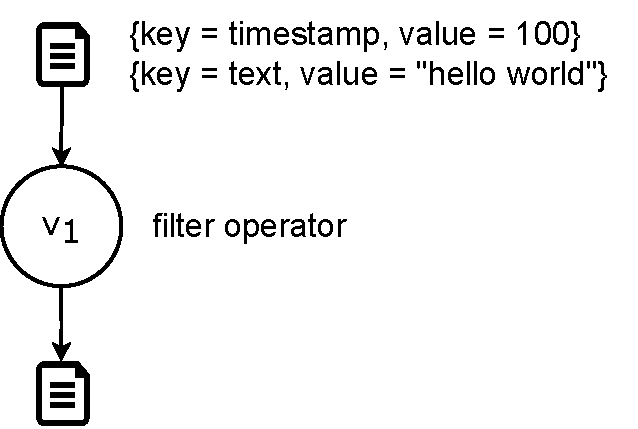
\includegraphics[scale=0.6]{figures/concepts/SPS-Stateless-Operator.pdf}
  \caption{An example of stateless operator.}
  \label{fig:sps-stateless-operator}
\end{figure}

Figure \ref{fig:sps-stateless-operator} presents an operator $\text{v}_1$ that performs a filtering task, which analyses if the text is in english written. If it is not, the event will not continue in the pipeline. In most cases, stateless operators are easily parallelizable, because it is not necessary to have consistency in the state of replicated operators, so they have a high scalability, which is useful for processing large amounts of data. When these operators are restarted, they have no impact in the overall processing of the data.

For stateful operators, the output depends on the internal state of the operator.  Therefore, they require past knowledge of the events or global state of the SPS to perform the task effectively. Such tasks are associated with windowed aggregations, pattern detection, or any operation that requires continuous analysis of data over some time.

\begin{figure}[ht!]
  \centering
   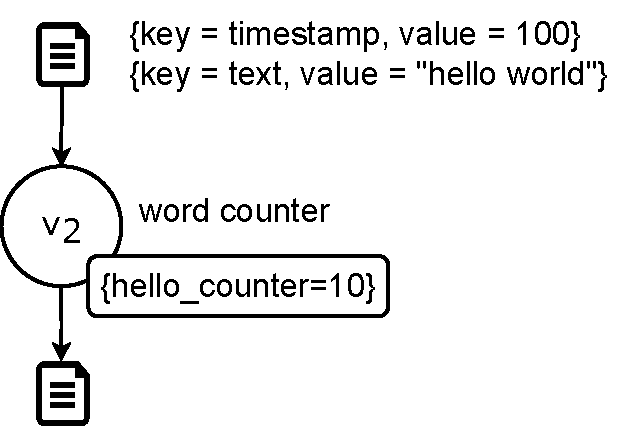
\includegraphics[scale=0.6]{figures/concepts/SPS-Stateful-Operator.pdf}
  \caption{An example of stateful operator.}
  \label{fig:sps-stateful-operator}
\end{figure}

Figure \ref{fig:sps-stateful-operator} presents operator $\text{v}_2$ which has a state that stores a counter indicating the number of tuples containing a specific word under a time window. Initially the operator $\text{v}_2$ has a state \texttt{hello\_counter=9}. Thus, after counting the incoming event the internal state will be \texttt{hello\_counter=10}. This state can be stored in memory or in an external database. The management of its state increases complexity, due to data consistency, fault tolerance, and scalability of the operator, because, as the number of replicas of this operator increases, it is necessary to ensure the consistency of the replica states.

\section{SPS Frameworks}
\label{sps-frameworks}
In this section, we will present two popular SPS frameworks: \textit{Storm} and \textit{Flink}. The logical architecture will be presented, with the components that make up the DAG, as well as the physical architecture, explaining the components necessary for its deployment and communication.

\subsection{Storm}

Storm \citep{toshniwal2014storm} is a distributed SPS framework implemented in Java and Clojure that enables the processing of unbounded streams of data. It was initially developed by the BackType team, which was later acquired by Twitter. It is an open-source Apache project, so there is a strong community of developers involved.

\subsubsection{Logical architecture}

A Storm application is represented by a DAG, also referred as \textit{Topology}. There are three types of components in a \textit{Topology}: \textit{Streams}, \textit{Spouts}, and \textit{Bolts}. 

\textit{Streams} are a sequence of tuples created and processed in parallel following the DAG model. These are distributed around the application. \textit{Streams} are composed of a structure of key-value tuples. Tuples can be defined by bytes, numbers, booleans or strings. Each \textit{Stream} must be declared by a unique identifier.

\textit{Spouts} are responsible for capturing the input data from external sources. They consume events and generate tuples sharing them to other \textit{Bolts} downstream in the \textit{Topology}. \textit{Spouts} can be implemented in either reliable or unreliable fashion. A reliable \textit{Spout} is capable of resending the same tuple in case it fails. Otherwise, it forgets to resend the tuple once it is emitted.

In \textit{Storm}, operators are called \textit{Bolts}. In general, these are lightweight tasks, so complex operations are designed as a pipeline of operators. \textit{Bolts} can receive the tuples emitted from one or more \textit{Streams}. Similarly to \textit{Spouts}, \textit{Bolts} can send the processed tuples through one or more \textit{Streams}. To guarantee processing, \textit{Bolts} can send an ACK (acknoledgement) message to indicate a tuple was processed. Each \textit{Bolt} is parallelizable, so it has an associated parallelism degree, which corresponds to the number of replicas of an operator.

\begin{figure}[!ht]
    \centering
    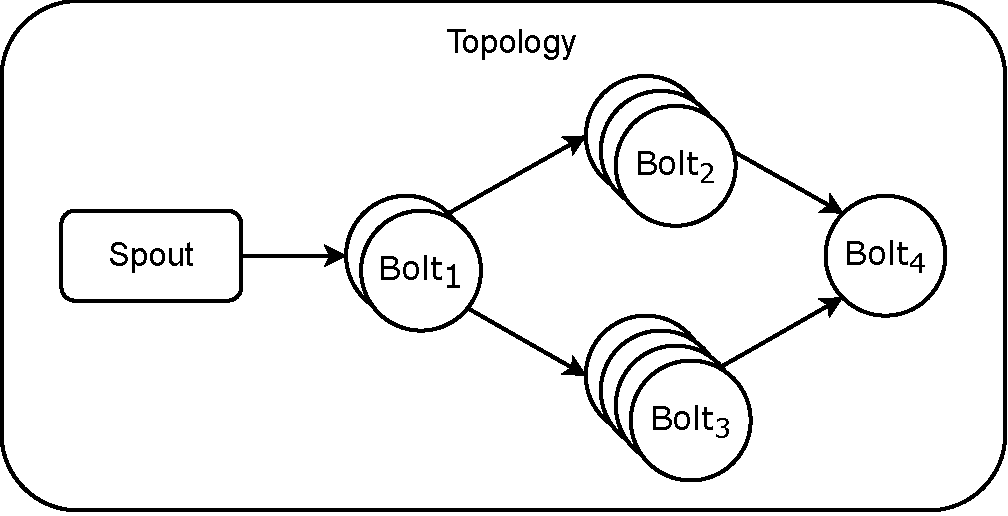
\includegraphics[width=0.75\textwidth]{figures/concepts/Storm-Logical.pdf}
    \caption{A Storm \textit{Topology} and components.}
    \label{fig:storm-logical}
\end{figure}


Figure \ref{fig:storm-logical} shows an Storm \textit{Topology} (DAG) example, composed of \textit{Spout}, and four \textit{Bolts}. The number of replicas for $Bolt_1$, $Bolt_2$, $Bolt_3$ and $Bolt_4$ are $2$, $3$, $4$ and $1$ respectively. $Spout$ is in charge of sending the raw data to $Bolt_1$ by distributing the stream data input to each of $Bolt_1$'s replicas based on some stream grouping. After processing the tuple, $Bolt_2$ sends the processed tuple to $Bolt_2$ and $Bolt_3$, the following \textit{Bolts} downstream in the DAG. If there is not \textit{Bolt} downstream, we are in presence of a sink operator and dataflow is terminated. The last operator that processes the data in \textit{Topology} is $Bolt_4$.


In the presence of \textit{Bolt's} replicas in Figure \ref{fig:storm-logical}, \textit{Stream} is partitioned and shared among them as shown in Figure \ref{fig:storm-stream-grouping}, which is defined by \textit{Stream grouping}. Every \textit{Bolt}'s replica processes the received tuple and sends the processed tuple to the next based on some stream grouping. Therefore, for each defined \textit{Stream} it is necessary to define \textit{Stream grouping} for sending a tuple between two components.

\begin{figure}[!ht]
    \centering
    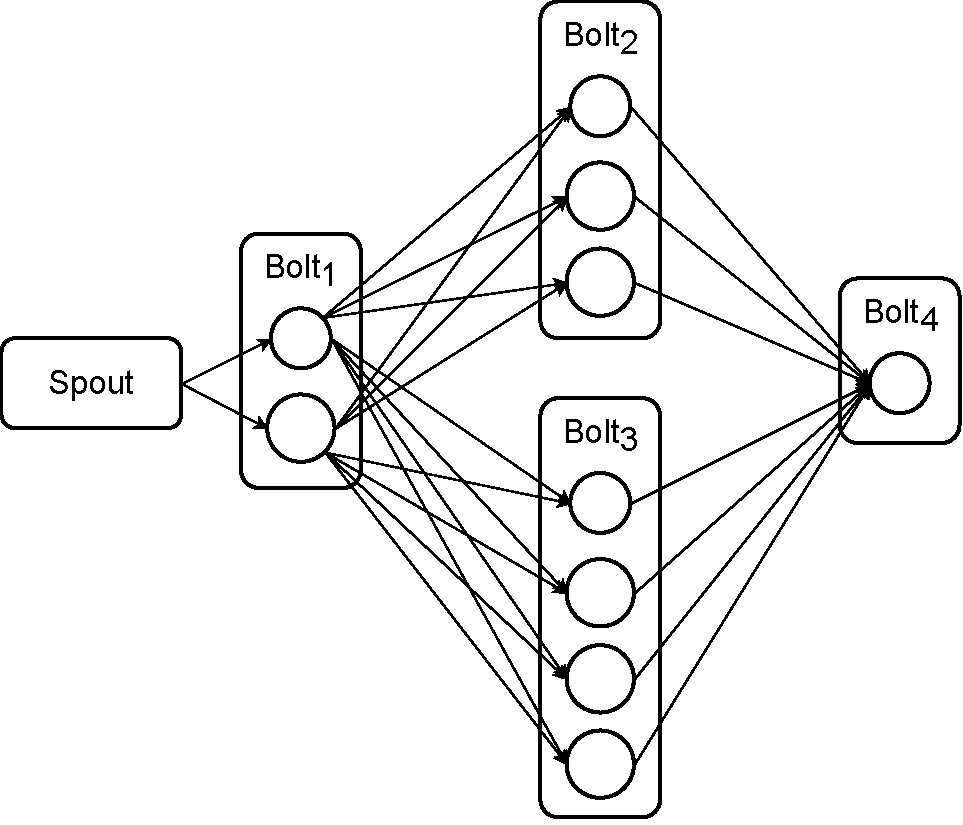
\includegraphics[width=0.75\textwidth]{figures/concepts/Storm-Stream-Grouping.pdf}
    \caption{Stream grouping in a Storm \textit{Topology}.}
    \label{fig:storm-stream-grouping}
\end{figure}

Storm has defined eight \textit{stream groupings}, can be used. If necessary, it is possible to define new \textit{stream groupings}.

\begin{enumerate}
\item \textit{Shuffle grouping}: Tuples are sent randomly to each replica.
\item \textit{Fields grouping}: The stream is partitioned by a field given in the tuple that determines which replica will receive the tuple.
\item \textit{Partial Key grouping}: This stream grouping is proposed by \cite{NasirMGKS15}. Similarly to \textit{Fields grouping}, it used a specific field for the choise of the replica, but also considers the load balancing between the available replicas.
\item \textit{All grouping}: Tuples are sent to all replicas.
\item \textit{Global grouping}: Tuples are sent to a single replica.
\item \textit{None grouping}: Tuples are sent randomly to each replica but in this case the same thread is always used by the assigned \textit{Bolts}.
\item \textit{Direct grouping}: Tuples are sent directly to the desired replica according to some attribute declared in \textit{Stream}.
\item \textit{Local grouping}: Tuples are sent to a group of replicas sharing the same resources.
\end{enumerate}

Except \textit{Partial Key grouping}, the drawback of these approaches is the potential lack of load balance. To cope with such a problem, other existing SPS propose hash-based data partition\citep{ShahHCF03}, partial-key based \citep{NasirMGKS15} or executor-centric solutions \citep{WangFMWZ19}.

Storm parallelism implementation is based on three concepts: \textit{Tasks}, \textit{Executors} and \textit{Worker processes}.

\textit{Tasks} are defined as data processing units, being replicas of a \textit{Bolt} or \textit{Spout}. While by default a task is assigned to one thread, it is possible to assign several tasks to the same thread.

An \textit{Executor} is a thread. One or more \textit{Tasks} of the same type (\textit{Bolt} or \textit{Spout}) can be assigned within the \textit{Executor}.

\textit{Worker processes} are a subset of a \textit{Topology}, so its in charge to run a set of \textit{Executors}. A \textit{Worker process} is a physical JVM. Each \textit{Worker process} is assigned to a machine and allocated resources can be configured according to the latter.

Figure \ref{fig:storm-parallelism} shows the parallelism of the Storm \textit{Topology} of Figure \ref{fig:storm-logical}. The \textit{Topology} has three subsets represented by \textit{Workers processes}, which are distributed on physical machines. Each \textit{Bolt} and \textit{Spout} represent a \textit{Task}, and each \textit{Task} is associated with a single \textit{Executor}, except in the case of $Bolt_2$, where all \textit{Tasks} are associated with a \textit{Executor}. In summary, the number of associated threads for each \textit{Bolt} is $Bolt_1 = 2$, $Bolt_2 = 1$, $Bolt_3 = 3$ and $Bolt_4 = 1$.

\begin{figure}[!ht]
    \centering
    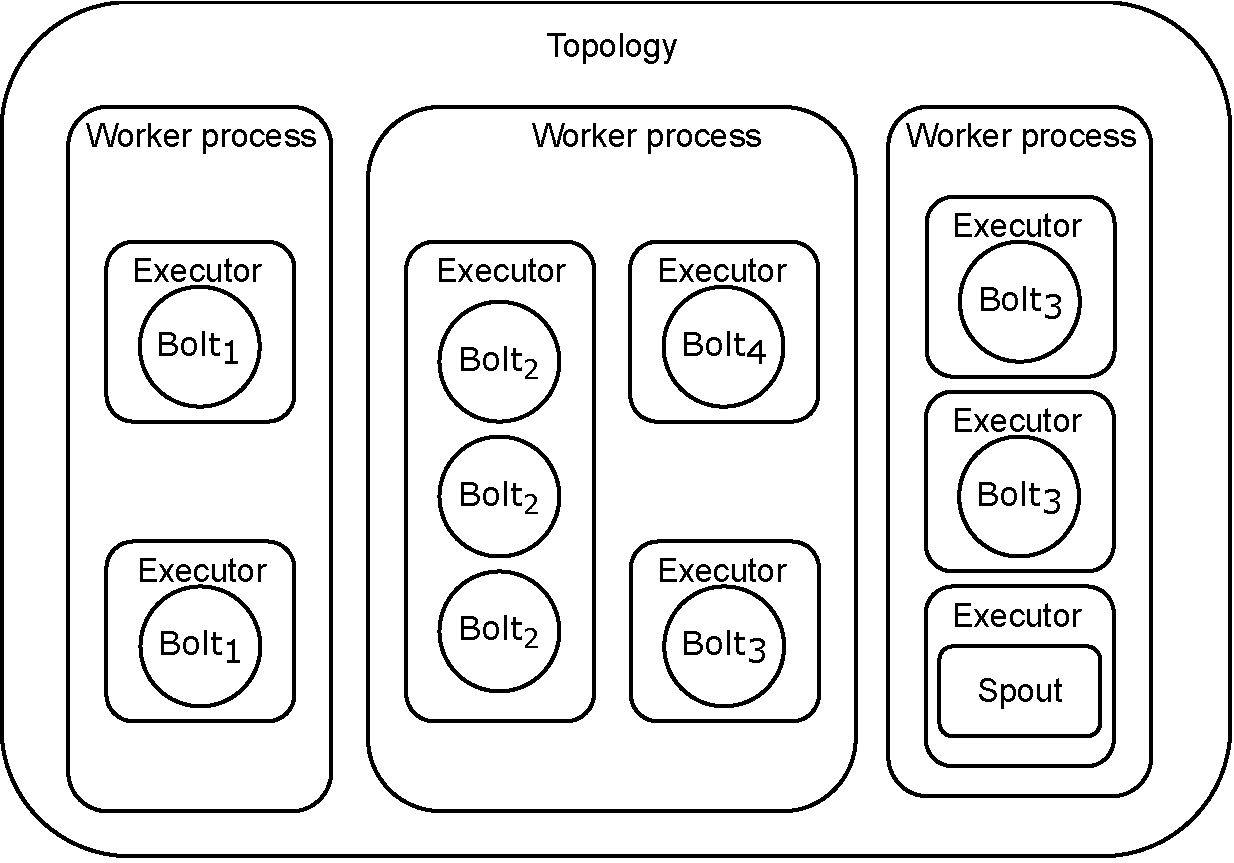
\includegraphics[width=0.75\textwidth]{figures/concepts/Storm-Logical-Parallelism.pdf}
    \caption{Parallelism of a Storm \textit{Topology}.}
    \label{fig:storm-parallelism}
\end{figure}

\subsubsection{Physical architecture}

Storm \textit{Topology} is deployed in a \textit{Storm Cluster}, which is a physical environment for its execution. Its components, hosted on machines, cores or VMs, are distributed on a platform such as a Grid, Cluster or Cloud. There are two kinds of components: \textit{Worker node} and  \textit{Master node}.

The \textit{Worker node} is responsible for hosting Storm \textit{Topology} tasks. Each \textit{Worker node} runs a daemon called \textit{Supervisor}. The role of the \textit{Supervisors} is to host one or more \textit{Worker processes}, so they deploy a subset of Storm \textit{Topology}. Thus, when deploying a Storm \textit{Topology} on a set of \textit{Worker processes}, each associated task will be distributed around \textit{Storm Cluster}.

The master node runs a daemon called \textit{Nimbus}, which is responsible for distributing the associated Storm \textit{Topology} code around the \textit{Storm Cluster}. At the same time, \textit{Nimbus} detects distributed component failures (i.e. node crashes or loss of messages) and the state of nodes. Finally, \textit{Nimbus} runs the scheduling algorithm.

The scheduling algorithm is in charge of performing the mapping. This case, load balance problems may arise. For instance, when a random policy is applied (as Storm can do it), there is no guarantee that the workload will be homogeneously distributed among the operators since an operator may be more complex than another one \cite{XingZH05} and machine resources could be heterogeneous.  Even with homogeneous computation nodes, load balance issues can also arise \cite{XuCTS14}. 
Figure \ref{fig:storm-physical} shows the scheduling of \textit{Storm Topology} (shown in Figure \ref{fig:storm-logical}) in a physical platform. According to some scheduling algorithms, each operator replica is placed in an available \textit{worker node}.

\begin{figure}[!ht]
     \centering
     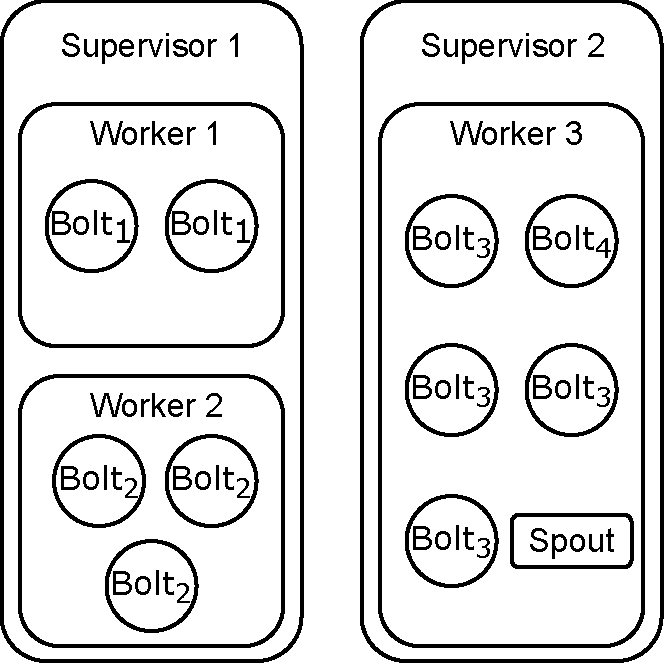
\includegraphics[width=0.45\textwidth]{figures/concepts/Storm-Physical.pdf}
     \caption{Storm physical architecture.}
     \label{fig:storm-physical}
\end{figure}

\subsubsection{Architecture}

For coordination between \textit{Nimbus} and the \textit{Supervisors}, \textit{Storm Cluster} uses \textit{Zookeeper}. Additionally, the states of the latter are stored in \textit{Zookeeper} or on a local disk, to provide fault tolerance in case of node failure.

Finally, \textit{Storm} architecture comprises \textit{Storm Cluster} and \textit{Zookeeper} cluster as shown by Figure \ref{fig:storm-architecture}.

\begin{figure}[!ht]
     \centering
     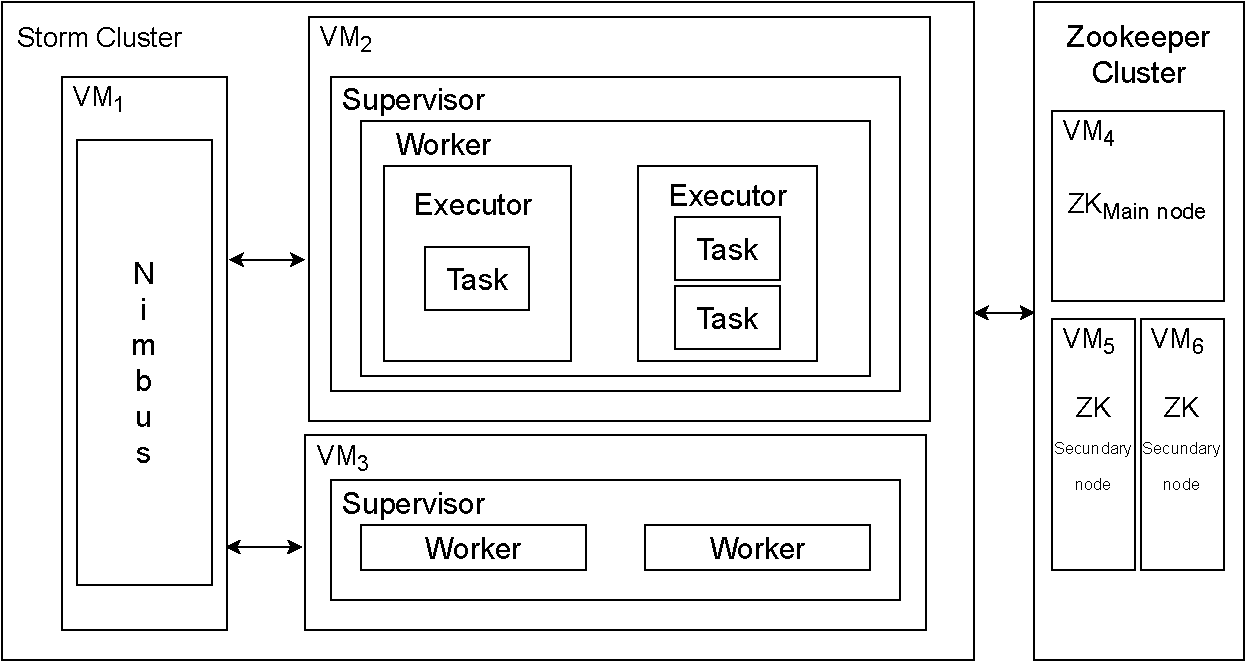
\includegraphics[width=0.8\textwidth]{figures/concepts/Storm-Architecture.pdf}
     \caption{Storm architecture.}
     \label{fig:storm-architecture}
\end{figure}

\subsection{Flink}
Flink \cite{Katsifodimos2016Flink} is a distributed SPS framework implemented in Java and Scala that enables the processing of unbounded data streams. It was initially developed by TU Berlin, and is currently part of the Stratosphere project.

\subsubsection{Logical architecture}

Like \textit{Storm}, a \textit{Flink Application} is a DAG. There are two types of components in a \textit{Flink Application}: \textit{Sources} and \textit{Operators}.

\textit{Sources} are the components necessary for sending external data to \textit{Flink Application}. Each \textit{Source} can be associated with logs, written data to external sinks, message queues, and interface with other systems. In this way, a \textit{Flink Application} can have one or more Sources in the data processing.

\textit{Operators} are the components that process the data in the \textit{Flink application} pipeline. Unlike \textit{Storm}, \textit{Flink} provides a high-level model, providing several default functions, which can be used. In this way, the system provides a high level of abstraction, simplifying various aspects of application construction. Like \textit{Storm}, each \textit{Operator} can be parallelised according to the application's requirements.

\begin{figure}[!ht]
    \centering
    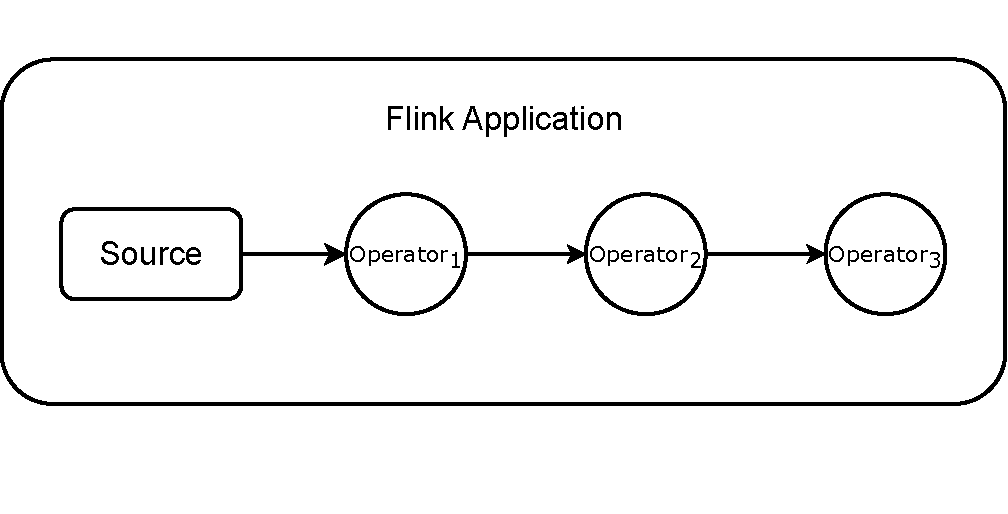
\includegraphics[width=0.75\textwidth]{figures/concepts/Flink-Logical.pdf}
    \caption{A Flink \textit{Topology}.}
    \label{fig:flink-logical}
\end{figure}

Figure \ref{fig:flink-logical} shows a \textit{Flink Application} (DAG) example, composed of a \textit{Source}, and three \textit{Operators}. In this example, can observe that the first \textit{Operator} performs the mapping task, while the second \textit{Operator} groups by a key and operates in a time window. These \textit{Operators} are named \textit{Transformation Operators}. After, the third \textit{Operator}, the last one, sends the processed data to either a database or an external system. This type of \textit{Operator} is called \textit{Sink Operator}.

\subsubsection{Physical architecture}

A \textit{Flink application} is deployed on \textit{Flink Cluster}, which has two components: \textit{Job Manager} and \textit{Task Manager}.

The \textit{Job Manager} is responsible for distributing and coordinating the execution of the \textit{Flink Application}. It decides on which machine each \textit{Task} will be deployed. At the same time, it monitors the status of the tasks, in case of a possible failure or progress in the stream, as well as the coordination of checkpoints and their recovery.

\textit{Task Manager} is the component that hosts one or more \textit{Tasks} of \textit{Flink Application}. Each \textit{Task} is associated to an \textit{Operator}, so this component must also allocate resources for its parallelisation. It also sends the state of the \textit{Tasks} to the \textit{Job Manager}.

Outside the \textit{Flink Cluster}, there is a component named \textit{Client}, which is responsible for the code of the \textit{Flink application} and for sending it to the \textit{Job Manager} for deployment. This component also receives statistics, results and the state of the execution of \textit{Flink Application}.

\begin{figure}[!ht]
     \centering
     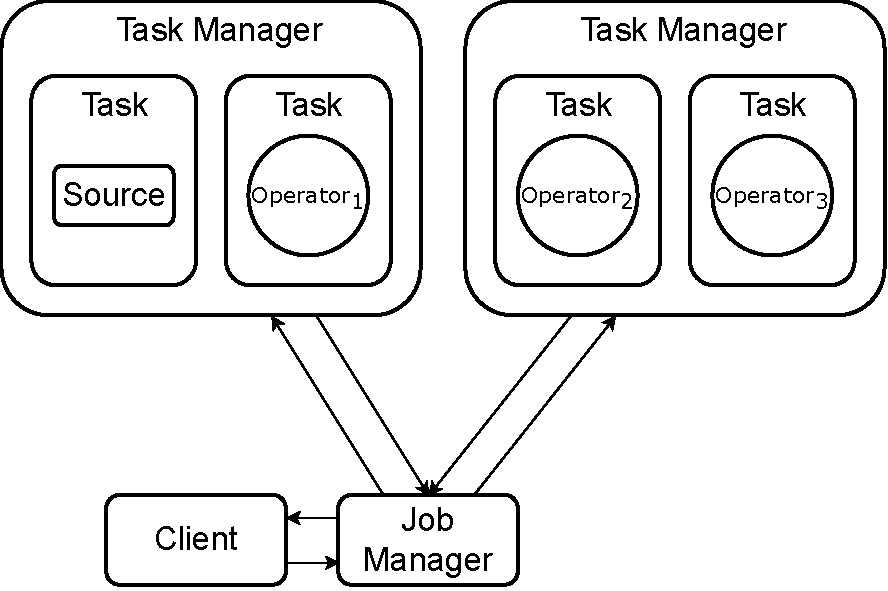
\includegraphics[width=0.7\textwidth]{figures/concepts/Flink-Physical.pdf}
     \caption{Flink physical architecture.}
     \label{fig:flink-physical}
\end{figure}

Figure \ref{fig:flink-physical} shows the scheduling of the \textit{Flink Application} (shown in Figure \ref{fig:flink-logical}) in a physical platform. According to some scheduling algorithms, each \textit{Operators} is placed in an available \textit{Task}.

\subsection{Discussion}
Although there are differences at the programming level, because \textit{Storm} does not provide a high level of abstraction as \textit{Flink}, both the logical and physical architecture are quite similar. On the one hand, the logical architecture is based on a DAG model, where each vertex is a component that performs a function and the edges are the data stream. As for the physical architecture, both are based on a model of main and secondary nodes, whereby the former is in charge of distributing the DAG as well as monitoring its state, and the later are responsible for processing the data.

It is worth noting that while we have given two examples, there have been other SPS frameworks, such as \textit{Apache S4} \citep{NeumeyerRNK10}, \textit{Apache Heron} \citep{KulkarniBFKKMPR15} or \textit{Apache Apex} \citep{GundabattulaW19}, but they have been given up over time. One of the main reasons is the flexibility provided by cloud services such as \textit{Amazon Web Services}, \textit{Google Cloud Platform} or \textit{Microsoft Azure}, where they provide their own SPS (\textit{Amazon Kinesis Data Streams}, \textit{Google Cloud Dataflow} and \textit{Microsoft Azure Stream Analytics}), with a high level of abstraction, simplifying both deployment and programming.

\section{Conclusion}
In this chapter, we present the concepts used in an SPS, as well as its requirements. We have explained each component, i.e. \textit{Stream}, \textit{Operator}, and \textit{Tuple}, and the concept of \textit{DAG}, which is the theoretical basis of the paradigm. In addition, we explained the parallelism of the operators, detailing their implementation and replication, as well as the types of \textit{Operator}, \textit{stateful} and \textit{stateless}, which are differentiated by the state handling in them. Finally, we present two SPS frameworks, \textit{Storm} and \textit{Flink}, explaining both their logical and physical architecture, as well as a discussion of the differences and similarities between them.